\documentclass{article}
\usepackage{amsmath}
\usepackage{amssymb}
\usepackage{bm}
\usepackage{amsthm}
\usepackage{enumerate}
\usepackage{graphicx}
\usepackage{psfrag}
\usepackage{color}
\usepackage{url}
\usepackage{listings}
\usepackage{xcolor}
\usepackage{tikz}
\usetikzlibrary{positioning}
\tikzset{main node/.style={circle,fill=gray!20,draw,minimum size=.5cm,inner sep=0pt},}

\definecolor{codegreen}{rgb}{0,0.5,0}
\definecolor{codewhite}{rgb}{1,1,1}
\definecolor{codegray}{rgb}{0.5,0.5,0.5}
\definecolor{codepurple}{rgb}{0.58,0,0.82}
\definecolor{codeblack}{rgb}{0,0,0}
\definecolor{codeorange}{rgb}{0.8,0.4,0}

\lstdefinestyle{mystyle}{
    backgroundcolor=\color{codewhite},   
    commentstyle=\color{codegray},
    keywordstyle=\color{codegreen},
    numberstyle=\color{codegray},
    stringstyle=\color{codeorange},
    basicstyle=\ttfamily ,
    breakatwhitespace=false,         
    breaklines=true,                 
    captionpos=b,                    
    keepspaces=true,                 
    numbers=left,                    
    numbersep=5pt,                  
    showspaces=false,                
    showstringspaces=false,
    showtabs=false,                  
    tabsize=4
}
\lstset{style=mystyle}


\setlength{\hoffset}{-1in}
\addtolength{\textwidth}{1.5in}
\setlength{\voffset}{-1in}
\addtolength{\textheight}{1.5in}
\newcommand{\be}{\begin{enumerate}}
\newcommand{\ee}{\end{enumerate}}
\newcommand{\BigO}[1]{\ensuremath\mathcal{O}\left(#1\right)}
\newcommand{\il}[1]{\lstinline!#1!}
\newcommand{\gnorm}[1]{\left|\left|#1\right|\right|}


\begin{document}
	\begin{center}
		\textbf{Spring 2020, CS 310:\ Homework 3 \& 4} \\
		\textbf{Due:\ Friday, March 27th, 2020} \\
		\textbf{Joseph Diaz: 819947915}
	\end{center}
\noindent\makebox[\linewidth]{\rule{\paperwidth}{0.4pt}}
\be[1.]
	\item Assume this tree is a Binary Search Tree even though you cannot see what the keys and values are at the nodes (the letters we write below are just ``names'' for the nodes for the purpose of answering the questions). 
	\begin{figure}[h]
	\centering
  	\includegraphics[width=.5\linewidth]{"BST".jpg}
	\end{figure}
	\be[a.]
		\item The value of H is greater than the value of I (True/False)\\
		False
		
		\item This Binary Search Tree is complete (True/False)\\
		False
		
		\item What is the height of the tree?\\
		5
		
		\item What is the maximum number of nodes that could be added to the tree without increasing its height?\\
		The height of this BST is 4, so the maximum number of nodes this tree can contain without increasing the height is $2^{4+1} - 1 = 31$. There 13 nodes in the tree already, so 18 more nodes could be added.
		
	\ee
	
	\item Suppose there is a Binary Min-Heap with exactly 4 nodes, containing items with priorities 3, 9, 11, and 15. 
	\be[a.] 
		\item Show every possible binary min-heap that could match this description. For each, draw the appropriate tree and the array representation. (You can show just the priorities, not the corresponding items.)
	\begin{center}
	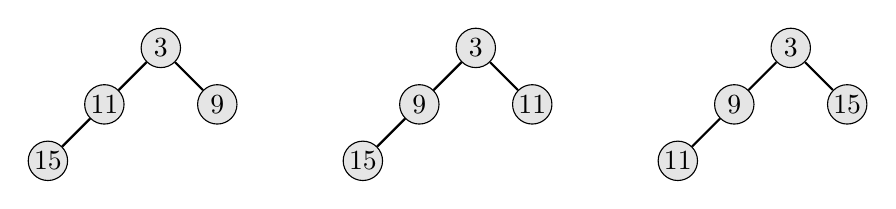
\begin{tikzpicture}
	\begin{scope}[xshift=-4cm]
    \node[main node] (1) {3};
    \node[main node] (2) [below left = .5cm  of 1] {11};
    \node[main node] (3) [below right = .5cm  of 1] {9};
    \node[main node] (4) [below left = .5cm  of 2] {15};
    

    \path[draw,thick]
    (1) edge node {} (2)
    (1) edge node {} (3)
    (4) edge node {} (2)
    ;
    \end{scope}
    
    \begin{scope}[xshift=0cm]
    \node[main node] (1) {3};
    \node[main node] (2) [below left = .5cm  of 1] {9};
    \node[main node] (3) [below right = .5cm  of 1] {11};
    \node[main node] (4) [below left = .5cm  of 2] {15};
    

    \path[draw,thick]
    (1) edge node {} (2)
    (1) edge node {} (3)
    (4) edge node {} (2)
    ;
    \end{scope}
    
    \begin{scope}[xshift=4cm]
    \node[main node] (1) {3};
    \node[main node] (2) [below left = .5cm  of 1] {9};
    \node[main node] (3) [below right = .5cm  of 1] {15};
    \node[main node] (4) [below left = .5cm  of 2] {11};
    

    \path[draw,thick]
    (1) edge node {} (2)
    (1) edge node {} (3)
    (4) edge node {} (2)
    ;
    \end{scope}
	\end{tikzpicture}
	\end{center}
	$$\Big[3,11,9,15\Big] \qquad\qquad\qquad \Big[3,9,11,15\Big] \qquad\qquad\qquad \Big[3,9,15,11\Big]$$
		\item For one of your answers to part (a), show what happens with 4 deleteMin operations. Clearly indicate which heap you are starting with and show the heap after each deleteMin. You can just draw the tree (not the array) after each step.\\
		Let us consider the left most of the 3 heaps above: 
		\begin{center}
	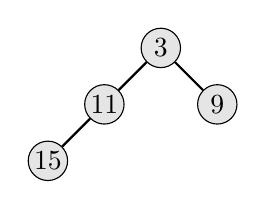
\begin{tikzpicture}
	\begin{scope}[xshift=-4cm]
    \node[main node] (1) {3};
    \node[main node] (2) [below left = .5cm  of 1] {11};
    \node[main node] (3) [below right = .5cm  of 1] {9};
    \node[main node] (4) [below left = .5cm  of 2] {15};
    

    \path[draw,thick]
    (1) edge node {} (2)
    (1) edge node {} (3)
    (4) edge node {} (2)
    ;
    \end{scope}
    
	\end{tikzpicture}
	\end{center}
	After the first deletion:
	\begin{center}
	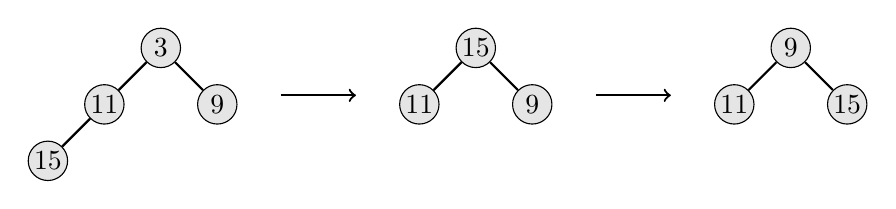
\begin{tikzpicture}
	\begin{scope}[xshift=-4cm]
    \node[main node] (1) {3};
    \node[main node] (2) [below left = .5cm  of 1] {11};
    \node[main node] (3) [below right = .5cm  of 1] {9};
    \node[main node] (4) [below left = .5cm  of 2] {15};
    

    \path[draw,thick]
    (1) edge node {} (2)
    (1) edge node {} (3)
    (4) edge node {} (2)
    ;
    \end{scope}
    
	\begin{scope}[xshift=-2cm]
    \node[] (1) {};
    \node[] (2) [below left = .5cm  of 1] {};
    \node[] (3) [below right = .5cm  of 1] {};
    

    \path[draw,->, thick]
    (2) edge node {} (3)
    ;
    \end{scope}
    
    \begin{scope}[xshift=0cm]
    \node[main node] (1) {15};
    \node[main node] (2) [below left = .5cm  of 1] {11};
    \node[main node] (3) [below right = .5cm  of 1] {9};
    

    \path[draw,thick]
    (1) edge node {} (2)
    (1) edge node {} (3)
    ;
    \end{scope}    
    
    \begin{scope}[xshift=2cm]
    \node[] (1) {};
    \node[] (2) [below left = .5cm  of 1] {};
    \node[] (3) [below right = .5cm  of 1] {};
    

    \path[draw,->, thick]
    (2) edge node {} (3)
    ;
    \end{scope}
    
    \begin{scope}[xshift=4cm]
    \node[main node] (1) {9};
    \node[main node] (2) [below left = .5cm  of 1] {11};
    \node[main node] (3) [below right = .5cm  of 1] {15};
    

    \path[draw,thick]
    (1) edge node {} (2)
    (1) edge node {} (3)
    ;
    \end{scope}    
	\end{tikzpicture}
	\end{center}
	
	After the second deletion:
	\begin{center}
	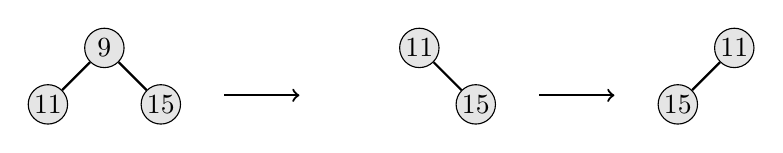
\begin{tikzpicture}
	\begin{scope}[xshift=-4cm]
    \node[main node] (1) {9};
    \node[main node] (2) [below left = .5cm  of 1] {11};
    \node[main node] (3) [below right = .5cm  of 1] {15};
    

    \path[draw,thick]
    (1) edge node {} (2)
    (1) edge node {} (3)
    ;
    \end{scope}    
    
	\begin{scope}[xshift=-2cm]
    \node[] (1) {};
    \node[] (2) [below left = .5cm  of 1] {};
    \node[] (3) [below right = .5cm  of 1] {};
    

    \path[draw,->, thick]
    (2) edge node {} (3)
    ;
    \end{scope}
    
    \begin{scope}[xshift=0cm]
    \node[main node] (1) {11};
    \node[main node] (2) [below right = .5cm  of 1] {15};

    

    \path[draw,thick]
    (1) edge node {} (2)
    ;
    \end{scope}    
    
    \begin{scope}[xshift=2cm]
    \node[] (1) {};
    \node[] (2) [below left = .5cm  of 1] {};
    \node[] (3) [below right = .5cm  of 1] {};
    

    \path[draw,->, thick]
    (2) edge node {} (3)
    ;
    \end{scope}
    
    \begin{scope}[xshift=4cm]
    \node[main node] (1) {11};
    \node[main node] (2) [below left = .5cm  of 1] {15};

    

    \path[draw,thick]
    (1) edge node {} (2)
    ;
    \end{scope}    
       
	\end{tikzpicture}
	\end{center}
	
	After the third deletion:
	\begin{center}
	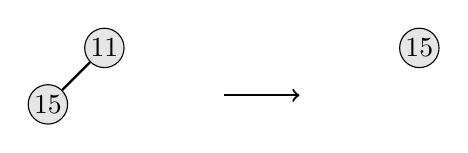
\begin{tikzpicture}
	\begin{scope}[xshift=-4cm]
    \node[main node] (1) {11};
    \node[main node] (2) [below left = .5cm  of 1] {15};
    
    

    \path[draw,thick]
    (1) edge node {} (2)
    ;
    \end{scope}    
    
	\begin{scope}[xshift=-2cm]
    \node[] (1) {};
    \node[] (2) [below left = .5cm  of 1] {};
    \node[] (3) [below right = .5cm  of 1] {};
    

    \path[draw,->, thick]
    (2) edge node {} (3)
    ;
    \end{scope}
    
    \begin{scope}[xshift=0cm]
    \node[main node] (1) {15};

    

    \path[draw,thick]
    ;
    \end{scope}    
	\end{tikzpicture}
	\end{center}
	and after the fourth deletion, our heap is empty.
	\ee
	
	\item For each of the following situations, name the best sorting algorithm we studied. (For one or two questions, there may be more than one answer deserving full credit, but you only need to give one answer for each.)\\
The array is mostly sorted already (a few elements are in the wrong place). 
	\be[a.] 
		\item You need an $\BigO{n \log(n)}$ sort even in the worst case and you cannot use any extra space except for a few local variables.\\
		Heapsort
		
		\item The data to be sorted is too big to fit in memory, so most of it is on disk.\\
		Insertion Sort
		
		\item You have many data sets to sort separately, and each one has only around 10 elements.\\
		Mergesort
		
		\item Instead of sorting the entire data set, you only need the $k$ smallest elements where $k$ is an input to the algorithm but is likely to be much smaller than the size of the entire data set.\\
		Quicksort
	\ee
	
	\item Draw the binary max heap that results from inserting 6,12,7,10,17,5,15 in that order into an initially empty binary min heap. You do not need to show the array representation of the heap. Draw all intermediate trees.\\
	\begin{center}
	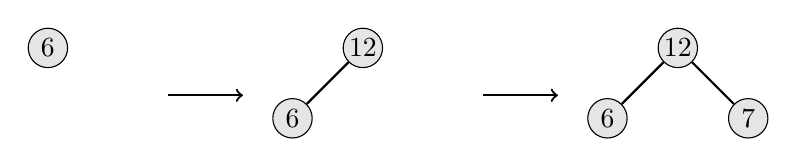
\begin{tikzpicture}
	\begin{scope}[xshift=-4cm]
    \node[main node] (1) {6};
    
    

    \path[draw,thick]
    ;
    \end{scope}
    
	\begin{scope}[xshift=-2cm]
    \node[] (1) {};
    \node[] (2) [below left = .5cm  of 1] {};
    \node[] (3) [below right = .5cm  of 1] {};
    

    \path[draw,->, thick]
    (2) edge node {} (3)
    ;
    \end{scope}
    
    \begin{scope}[xshift=0cm]
    \node[main node] (1) {12};
    \node[main node] (2) [below left = .75cm  of 1] {6};
    

    \path[draw,thick]
    (1) edge node {} (2)
    ;
    \end{scope}    
    
    \begin{scope}[xshift=2cm]
    \node[] (1) {};
    \node[] (2) [below left = .5cm  of 1] {};
    \node[] (3) [below right = .5cm  of 1] {};
    

    \path[draw,->, thick]
    (2) edge node {} (3)
    ;
    \end{scope}
    
    \begin{scope}[xshift=4cm]
    \node[main node] (1) {12};
    \node[main node] (2) [below left = .75cm  of 1] {6};
    \node[main node] (3) [below right = .75cm  of 1] {7};
    
    

    \path[draw,thick]
    (1) edge node {} (2)
    (1) edge node {} (3)
    ;
    \end{scope}    
	\end{tikzpicture}
	\end{center}
	\begin{center}
	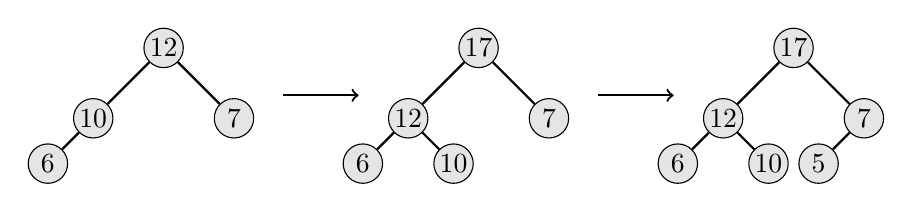
\begin{tikzpicture}
	\begin{scope}[xshift=-4cm]
    \node[main node] (1) {12};
    \node[main node] (2) [below left = .75cm  of 1] {10};
    \node[main node] (3) [below right = .75cm  of 1] {7};
    \node[main node] (4) [below left = .3cm  of 2] {6};
    

    \path[draw,thick]
    (1) edge node {} (2)
    (1) edge node {} (3)
    (4) edge node {} (2)
    ;
    \end{scope}
    
	\begin{scope}[xshift=-2cm]
    \node[] (1) {};
    \node[] (2) [below left = .5cm  of 1] {};
    \node[] (3) [below right = .5cm  of 1] {};
    

    \path[draw,->, thick]
    (2) edge node {} (3)
    ;
    \end{scope}
    
    \begin{scope}[xshift=0cm]
    \node[main node] (1) {17};
    \node[main node] (2) [below left = .75cm  of 1] {12};
    \node[main node] (3) [below right = .75cm  of 1] {7};
    \node[main node] (4) [below left = .3cm  of 2] {6};
    \node[main node] (5) [below right = .3cm  of 2] {10};
    

    \path[draw,thick]
    (1) edge node {} (2)
    (1) edge node {} (3)
    (2) edge node {} (4)
    (2) edge node {} (5)
    ;
    \end{scope}    
    
    \begin{scope}[xshift=2cm]
    \node[] (1) {};
    \node[] (2) [below left = .5cm  of 1] {};
    \node[] (3) [below right = .5cm  of 1] {};
    

    \path[draw,->, thick]
    (2) edge node {} (3)
    ;
    \end{scope}
    
    \begin{scope}[xshift=4cm]
    \node[main node] (1) {17};
    \node[main node] (2) [below left = .75cm  of 1] {12};
    \node[main node] (3) [below right = .75cm  of 1] {7};
    \node[main node] (4) [below left = .3cm  of 2] {6};
    \node[main node] (5) [below right = .3cm  of 2] {10};
    \node[main node] (6) [below left = .3cm  of 3] {5};
    

    \path[draw,thick]
    (1) edge node {} (2)
    (1) edge node {} (3)
    (2) edge node {} (4)
    (2) edge node {} (5)
    (3) edge node {} (6)
    ;
    \end{scope}    
	\end{tikzpicture}
	\end{center}
	\begin{center}
	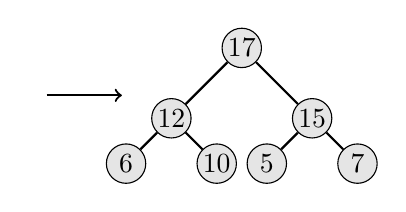
\begin{tikzpicture}
	\begin{scope}[xshift=-1cm]
    \node[] (1) {};
    \node[] (2) [below left = .5cm  of 1] {};
    \node[] (3) [below right = .5cm  of 1] {};
    

    \path[draw,->, thick]
    (2) edge node {} (3)
    ;
    \end{scope}
	\begin{scope}[xshift=1cm]
    \node[main node] (1) {17};
    \node[main node] (2) [below left = .75cm  of 1] {12};
    \node[main node] (3) [below right = .75cm  of 1] {15};
    \node[main node] (4) [below left = .3cm  of 2] {6};
    \node[main node] (5) [below right = .3cm  of 2] {10};
    \node[main node] (6) [below left = .3cm  of 3] {5};
    \node[main node] (7) [below right = .3cm  of 3] {7};


    \path[draw,thick]
    (1) edge node {} (2)
    (1) edge node {} (3)
    (2) edge node {} (4)
    (2) edge node {} (5)
    (3) edge node {} (6)
    (3) edge node {} (7)
    ;
    \end{scope}
    
	\end{tikzpicture}
	\end{center}
	
	\item Describe the most time-efficient way to implement the operations listed below. Assume no duplicate values and that you can implement the operation as a member function of the class – with access to the underlying data structure, including knowing the number of values currently stored $(N)$. Then, give the tightest possible upper bound for the worst case running time for each operation in terms of $N$.\\
	\textbf{For any credit, you must explain why it gets this worst case running time.}
	\be[a.] 
		\item Given a binary min heap, find which value is the minimum value and delete it. 
		\begin{proof}[Solution]
		As the heap in question is a binary min heap, removing the smallest element is $\BigO{1}$ as that element is at the root and replacing the root with the last node is also $\BigO{1}$. Ensuring that the heap property is maintained, though, is $\BigO{\log(N)}$, which is also the worst case running time.\\
		This is the worst case running time, because the approximate height of the heap is $\log(N)$, and maintaining the heap property (along with all relevant swaps and replacements) may require pushing the new root back towards the bottom as part of the down heap operation.
		\end{proof}
		
		\item Given a binary search tree, find which value is the minimum value and delete it.
		\begin{proof}[Solution]
		The operations required to find the minimum element are to traverse down the left child of each node (starting at the root) until the left most node is reached. That element will be the minimum element as we're working with a Binary Search Tree. After deleting that element no more operations will be required, as the structure of a BST will not be violated, and given that $\log(N)$ is the height of the tree, the worst case running time will be $\BigO{\log(N)}$ as in Part ~a.
		\end{proof}
	\ee


\ee
\noindent\makebox[\linewidth]{\rule{\paperwidth}{0.4pt}}
	
\end{document}
